Die mit dem X-Y-Schreiber aufgenommenen Kurven sind in den Abbildungen \ref{fig:Scan10}-\ref{fig:Scan30} zu sehen. Für jedes Kurvenpaar wird mit den Kalibrierungswerten aus Schritt \ref{Schritt6} des vorigen Kapitels ein Umrechnungsmaß berechnet. Die Stromstärken $I_1,I_2$ der Resonanzstellen und deren Ungenauigkeiten werden optisch abgeschätzt und dann mit Hilfe des Umrechnungsmaßes von \si{\centi\meter} in \si{\milli\ampere} umgerechnet, diese Werte sind in Tabelle \ref{tab:Werte} aufgetragen.
\begin{table}
    \centering
    \caption{Stromstärken $I_1,I_2$ beim Auftreten des Maximums für verschiedene Anregungsfrequenzen $\nu_e$ mit dem jeweiligen Skalierungsfaktor}
    \label{tab:Werte}
    \sisetup{parse-numbers=false}
    \begin{tabular}{
	S[table-format=2.3]
	S[table-format=3.0]
	@{${}\pm{}$}
	S[table-format=2.0, table-number-alignment = left]
	S[table-format=3.0]
	@{${}\pm{}$}
	S[table-format=2.0, table-number-alignment = left]
	S[table-format=2.1]
	@{${}\pm{}$}
	S[table-format=1.1, table-number-alignment = left]
	}
	\toprule
	{$\nu_e \ \mathrm{in} \ \si{\mega\hertz}$}		& \multicolumn{2}{c}{$I_1 \ \mathrm{in} \ \si{\milli\ampere}$}		& 
	\multicolumn{2}{c}{$I_2 \ \mathrm{in} \ \si{\milli\ampere}$}		& \multicolumn{2}{c}{Skala in \si{\milli\ampere\per\centi\meter}}		\\ 
	\midrule
    10.588 & 232 & 5  & 307 & 5  & 41.5 & 0.5 \\
15.970 & 357 & 9  & 407 & 5  & 16.7 & 0.3 \\
20.560 & 453 & 9  & 546 & 4  & 18.1 & 0.3 \\
23.870 & 587 & 10 & 633 & 10 & 15.2 & 0.6 \\
29.420 & 717 & 10 & 787 & 8  & 15.3 & 0.4 \\

    \bottomrule
    \end{tabular}
    \end{table}
 \\
Mit Hilfe von
\begin{align}
	B(I) = \frac{8}{\sqrt{125}}\frac{156}{\SI{0.1}{\meter}}\mu_0I
\end{align}
werden die Stromstärken in Flussdichten umgerechnet. Je nach Orientierung der Spule zum Erdmagnetfeld wird das Feld der Helmholtz-Spulen verstärkt oder abgeschwächt. Die Stärke des Erdfeldes ist demnach die Hälfte der Differenz der beiden Flussdichten. Pro eingestellter Frequenz ergibt sich so je eine magnetische Flussdichte des Erdmagnetfeldes, ihr Mittelwert ist
\[ B_\text{Erde} = \SI{0.047+-0.003}{\milli\tesla}
 \quad. \]
Der Mittelwert der beiden Flussdichten ergibt die vom erdmagnetfeld-bereinigte Flussdichte. Für jede Frequenz ist diese zusammen mit der Flussdichte des Erdmagnetfeldes in Tabelle \ref{tab:BFeld} dargestellt.
\begin{table}
    \centering
    \caption{Bei der Regression verwendete Werte}
    \label{tab:Regression}
    \sisetup{parse-numbers=false}
    \begin{tabular}{
	S[table-format=2.3]
	S[table-format=1.2]
	@{${}\pm{}$}
	S[table-format=1.2, table-number-alignment = left]
	}
	\toprule
	{$\nu \ \mathrm{in} \ \si{\mega\hertz}$}		& \multicolumn{2}{c}{$B \ \mathrm{in} \ \si{\milli\tesla}$}		\\ 
	\midrule
    10.588 & 0.378 & 0.005 & 0.052 & 0.005 \\
15.970 & 0.536 & 0.007 & 0.035 & 0.007 \\
20.560 & 0.701 & 0.007 & 0.065 & 0.007 \\
23.870 & 0.86  & 0.01  & 0.03  & 0.01  \\
29.420 & 1.055 & 0.009 & 0.049 & 0.009 \\

    \bottomrule
    \end{tabular}
    \end{table}
 \\
\clearpage
Zur Berechnung des Landé-Faktors wird in Anlehnung an Gleichung \eqref{eq:DeltaE} die Funktion
\begin{align*}
	B(\nu) = \frac{h}{g\mu_\text{B}}\nu
\end{align*}
an die Wertepaare $\{\nu_e,B\}$ aus Tabelle \ref{tab:BFeld} gefittet. Die Berechnung ergibt für den Fitparameter $g$ den Wert
\begin{align*}
	g = \SI{2.04+-0.03}{}
 \quad,
\end{align*}
Abbildung \ref{fig:fit} zeigt den Fit, die Messwerte und die Kurve, die mit dem Literaturwert $g = 2.0023$ \cite{gFaktor} erhalten wird. Auf das Einzeichnen der Fehlerbalken wird verzichtet, da sie aufgrund der kleinen Unsicherheiten in $B$ die Lesbarkeit beeinträchtigen.
\begin{figure}[h!]
	\centering
	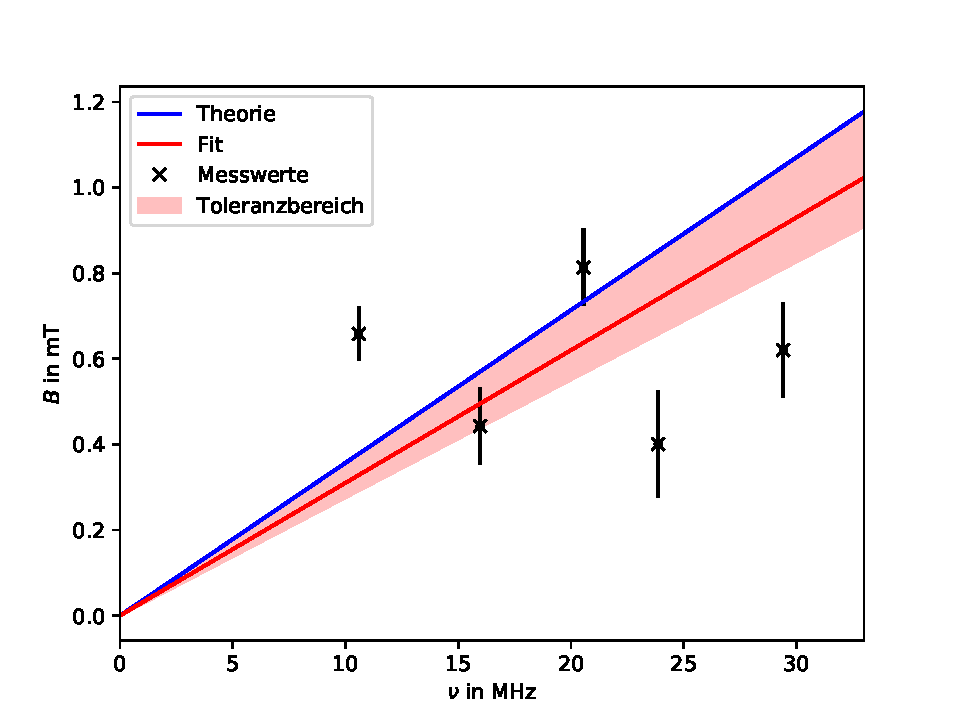
\includegraphics[width=0.8\textwidth]{Fit.pdf}
	\caption{Fit zur Bestimmung des Landé-Faktors}
	\label{fig:fit}
\end{figure}

\begin{figure}
	\centering
	\begin{subfigure}{0.5\textwidth}
		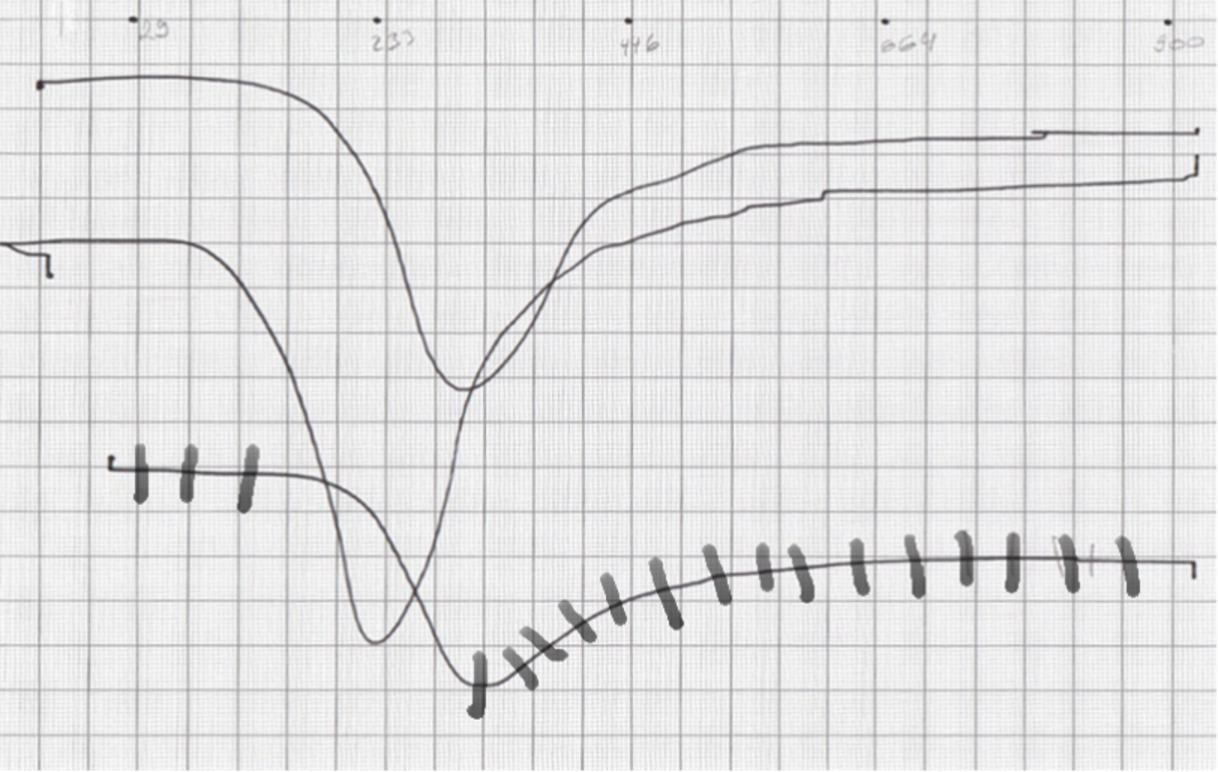
\includegraphics[width=\linewidth]{Scan10.pdf}
		\caption{\SI{10.588}{\mega\hertz}}
		\label{fig:Scan10} 
	\end{subfigure}
	\begin{subfigure}{0.5\textwidth}
		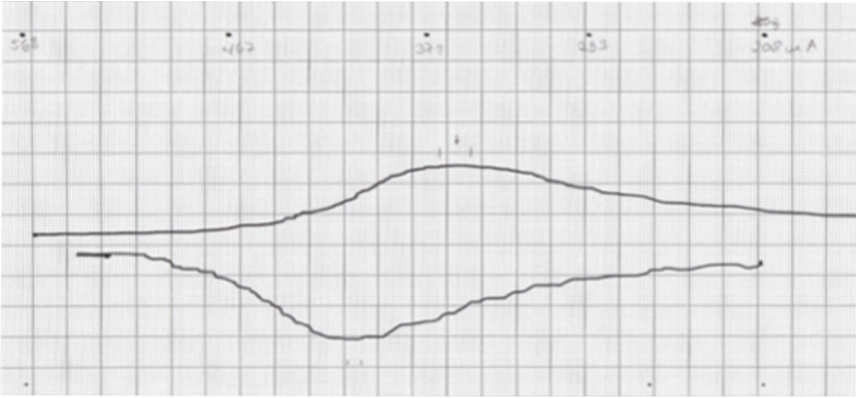
\includegraphics[width=\linewidth]{Scan15.pdf}
		\caption{\SI{15.970}{\mega\hertz}}
		\label{fig:Scan15}
	\end{subfigure}
	\begin{subfigure}{0.5\textwidth}
		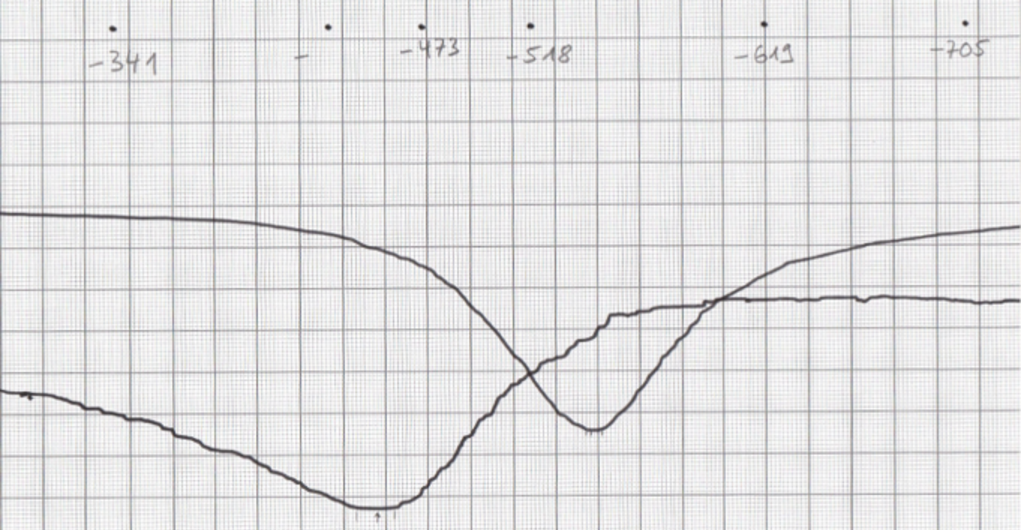
\includegraphics[width=1\linewidth]{Scan20.pdf}
		\caption{\SI{20.560}{\mega\hertz}}
		\label{fig:Scan20} 
	\end{subfigure}
	\begin{subfigure}{0.5\textwidth}
		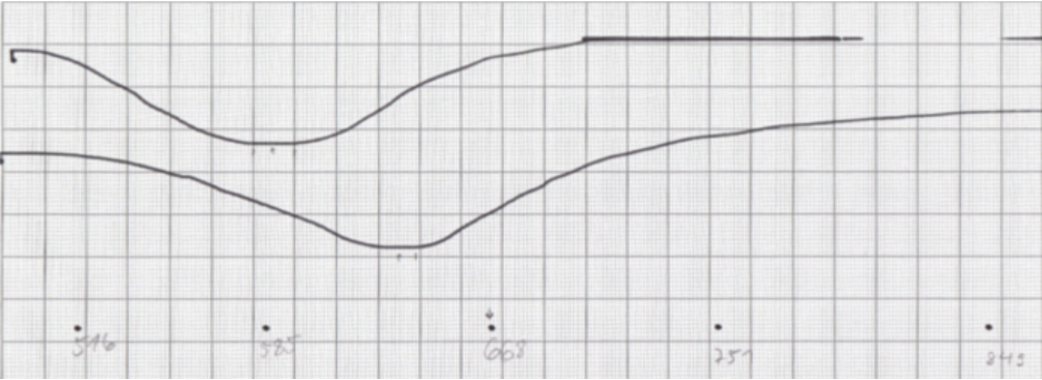
\includegraphics[width=1\linewidth]{Scan25.pdf}
		\caption{\SI{23.870}{\mega\hertz}}
		\label{fig:Scan25}
	\end{subfigure}
	\begin{subfigure}{0.5\textwidth}
		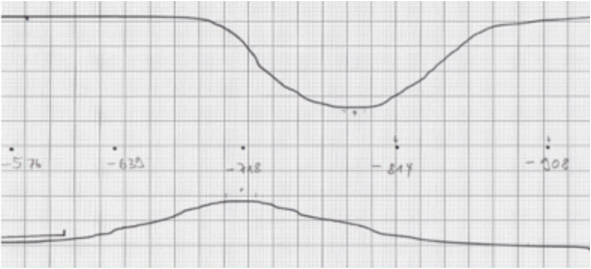
\includegraphics[width=1\linewidth]{Scan30.pdf}
		\caption{\SI{29.420}{\mega\hertz}}
		\label{fig:Scan30}
	\end{subfigure}
	\caption{Scans der Resonanzkurven}
\end{figure}
